\section{Introduction}
\label{sec:intro}

%While the number of items on e-commerce platforms grows dramatically day by day, 
%e-commerce giants like Alibaba and Amazon 
%are taking great efforts to 
%figure out which small set of items can satisfy users every time they open the shopping apps. 
%Personalized search and recommendation
%are two effective ways for those platforms
%to help their users quickly zoom into a small set of items 
%that meet their personal needs from an enormous candidate set. 
%However, user needs in e-commerce are still way behind satisfaction since there is a huge semantic gap between what users need in their mind and how the items are organized in e-commerce platforms.

One major functionality of e-commerce platforms is to match the shopping need of a customer to a small set of items from an enormous candidate set.
With the rapid developments of search engine and recommender system,
customers are able to quickly find those items they need.
However, the experience is still far from ``intelligent''.
One significant reason is that there exists a huge semantic gap between what users need in their mind and how the items are organized in e-commerce platforms.
The taxonomy to organize items in Alibaba (actually almost every e-commerce platforms) is generally based on \textbf{CPV} (Category-Property-Value):
thousands of categories form a hierarchical structure according to different granularity, and properties such as color and size are defined upon each leaf node.
It is a natural way of organizing and managing billions of items in nowadays e-commerce platform, and already becomes the essential component in downstream applications including search and recommendation.
However, existing taxonomies or ontologies in e-commerce are difficult to interpret various user needs comprehensively and accurately due to the semantic gap, which will be explained in the following two scenarios.

%The users come to an e-commerce platform can be roughly categorized into four types according to their particular needs.
%%\footnote{\url{https://medium.com/gobeyond-ai/the-coming-disruption-in-e-commerce-search-3ffa0eb9a5d9}}:
%1) users who has an exact product in mind, for example, a user who want to buy the newly released iPhone XI 256gb gold.
%2) Users who have a category of products in mind, for example, a customer who wants to buy a rice cooker or a refrigerator. However, he does not know which particular product has the right features he needs. Moreover, it is also possible that after some painstaking research, he may realize, instead of a rice cooker, what he really needs is a steamer.
%3) Users who have a situation or a problem but do not know what products can help, for example, a customer who is planning an outdoor barbecue, who is concerned with how to get rid of a raccoon in his garden, or who is panicking at the eleventh hour about a Valentine's day gift.
%4) Users who do not have anything in mind to buy. They just want to be informed, inspired, enlightened and entertained, but generally they just want to spend some time and have fun.
%How well are we stratify all those needs?
%\XS{The case of e-commerce search}
For years, e-commerce search engine is teaching our users how to input keywords wisely so that the wanted items can be quickly found. 
However, it seems keyword based searching only works for those users who know the exact product they want to buy. 
The problem is, users do not always know the exact product. 
More likely what they have in mind is a type or a category of products, with some extra features. 
Even worse, they only have a scenario or a problem but no idea what items could help. 
In these cases, a customer may choose to conduct some research outside the e-commerce platform to narrow down to an exact product, which harms the user experience and making e-commerce search engine not intelligent at all. 
If tracing back to the source, 
the real reason behind this is that existing ontologies in e-commerce doesn't contain structured knowledge indicating what products are needed for an ``outdoor barbecue'' 
or what is ``preventing the olds from getting lost''. 
Typing search queries like these inevitable leads to user needs mismatch and query understanding simply degenerates to key words matching.

\begin{figure*}[th]
	\centering
	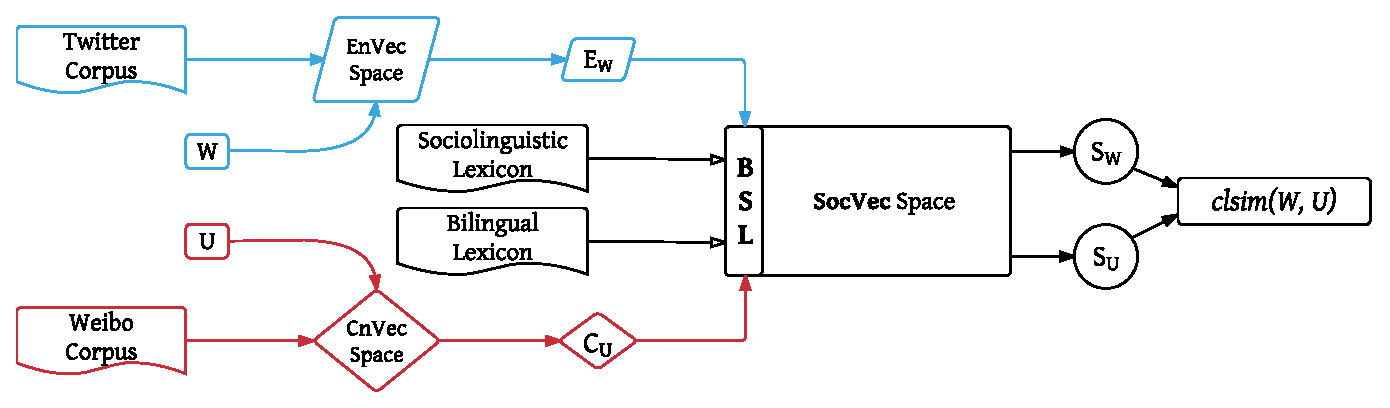
\epsfig{file=figures/overview.eps, width=2.1\columnwidth}
	\caption{Overview of ``AliCoCo'', which consists of four layers: e-commerce concepts, primitive concepts, taxonomy and items.}
	\label{fig:overview}
\end{figure*}



%\XS{The case of recommendation: also not driven by user needs}
The same problem exists in item recommendation. 
Due to the prohibitive size of transaction data in real-world industry scenario, recommendation algorithms widely adopt the 
idea of item-based CF \cite{sarwar2001item}, which
can recommend from very large set of options with relatively small amount of computation, 
depending on the pre-calculated similarity between item pairs.
The recommender system uses user's historical behaviors as triggers to recall a small set of most similar items as candidates, 
then recommends items with highest weights after scoring with a ranking model.
A critical shortcoming of this framework is that it is not driven by user needs in the first place, 
which inevitably leads to a dilemma where items recommended are hard to be explained 
except for trivial reasons such as ``similar to those items you have already viewed or purchased''.
Besides, it also prevents the recommender system from jumping out of 
historical behaviors to explore other implicit or latent user interests.
Therefore, despite the widespread of its use,
the performance of current recommendation systems is still under criticism. 
Users are complaining that some recommendation results are redundant and lack novelty, 
since current recommender systems can only satisfy very limited user needs such as the needs for a particular category or brand.
The lack of intermediate nodes in current e-commerce ontologies that can represent various user needs constrains the development of recommender systems.



In this paper, we attempt to bridge the semantic gap between actual user needs and existing ontologies in e-commerce platforms 
by building a new ontology towards universal user needs understanding.
It is believed that the cognitive system of human beings is based on \textit{concepts} \cite{murphy2002thebig,bloom2003glue},
and the taxonomy and ontology of concepts give humans the ability to understand \cite{wu2012probase}.
Inspired by it, we construct the ontology mainly based on concepts and name it ``\textbf{AliCoCo}'': \textbf{Co}gnitive \textbf{Co}ncept Net in \textbf{Ali}baba.
Different from most existing e-commerce ontologies, 
which only contain nodes such as categories or brands, 
a new type of node, e.g.,
``Outdoor Barbecue'' and ``Keep Warm for Kids'', is introduced as 
bridging concepts connecting user and items to satisfy some 
high-level user needs or shopping scenarios. 
%more than just needs for a category or a brand. 
Shown in the top of \figref{fig:overview}, we call these nodes ``\textbf{e-commerce concepts}'',
whose structure represents a set of items from different categories 
with certain constraints (more details in \secref{sec:ecommerce}) .
%\footnote{The constraints correspond to concept schema defined in \secref{sec:ecn}}.
%\KZ{Maybe need to say explicitly E-commerce Concept Net will be discussed
%separately by a different paper? Now it appears that you are going to
%introduce this net the first time in this paper.}
%These e-commerce concepts, together with categories, brands and items, 
%form a new kind of e-commerce knowledge graph, called
%\textbf{``AliCoCo''} (\figref{fig:kg} (a)). 
%\KZ{I think figure 2(a) can be included here instead. Don't refer to a fig in the later sections.}
%where concepts are related with representative categories, brands and items.
For example, ``Outdoor Barbecue'' is one such e-commerce concept,  
consisting of products such as grills, butter and so on, 
which are necessary items to host a successful outdoor barbecue party.
Therefore, AliCoCo is able to help search engine directly suggest a customer 
``items you will need for outdoor barbecue'' 
after he inputs keyword ``barbecue outdoor'',
or help recommender system remind him of preparing things that can ``keep warm for your kids'' as 
there will be a snowstorm coming next week.



%\XS{Applications in recommendation}
%Once user needs are inferred accurately, various recommender 
%systems can be benefited.
There are several possible practical scenarios in which 
applying such e-commerce concepts can be useful.
The first and most natural scenario is directly displaying those concepts to users 
together with its associated items.
\figref{fig:cloud}(a/b) shows the real implementation of this idea in 
\textit{Taobao} \footnote{\url{http://www.taobao.com}} App.
%the largest Chinese e-commerce platform. 
Once a user typing ``Baking'' (a), 
he will enter into a page (right) where different items for baking are displayed, making the search experience a bit more intelligent.
It can also be integrated into recommender systems.
Among normal recommended items, 
concept ``Tools for Baking'' is displayed to users as a card with its name and the picture of a representative item (b).
Once a user clicks on it, he will enter into the page on the right.
In this way, the recommender system is acting like a salesperson in a shopping mall, 
who tries to guess the needs of his customer and and then suggests how to satisfy
them. 
If their needs are correctly inferred, users are more likely to accept 
the recommended items.
%Another scenario is intelligent search, where search queries are associated with most possible concepts at first. In \figref{fig:cloud}(b), search query ``Baking'' triggered the concept card ``Tools for baking'' with  
%related items.
Other scenarios can be providing explanations in search or recommendation as 
shown in \figref{fig:cloud}(c).
While explainable recommendation attracts much research attention 
recently \cite{zhang2018explainable}, 
most existing works are not practical enough for industry systems,
since they are either too complicated 
(based on NLG \cite{zanker2010knowledgeable,cleger2012explaining}), or too trivial 
(e.g., ``how many people also viewed'' \cite{costa2018automatic,li2017neural}).
Our proposed concepts, on the contrary, precisely conceptualize user needs and are
easy to understand.

 \begin{figure}[th]
	\centering
	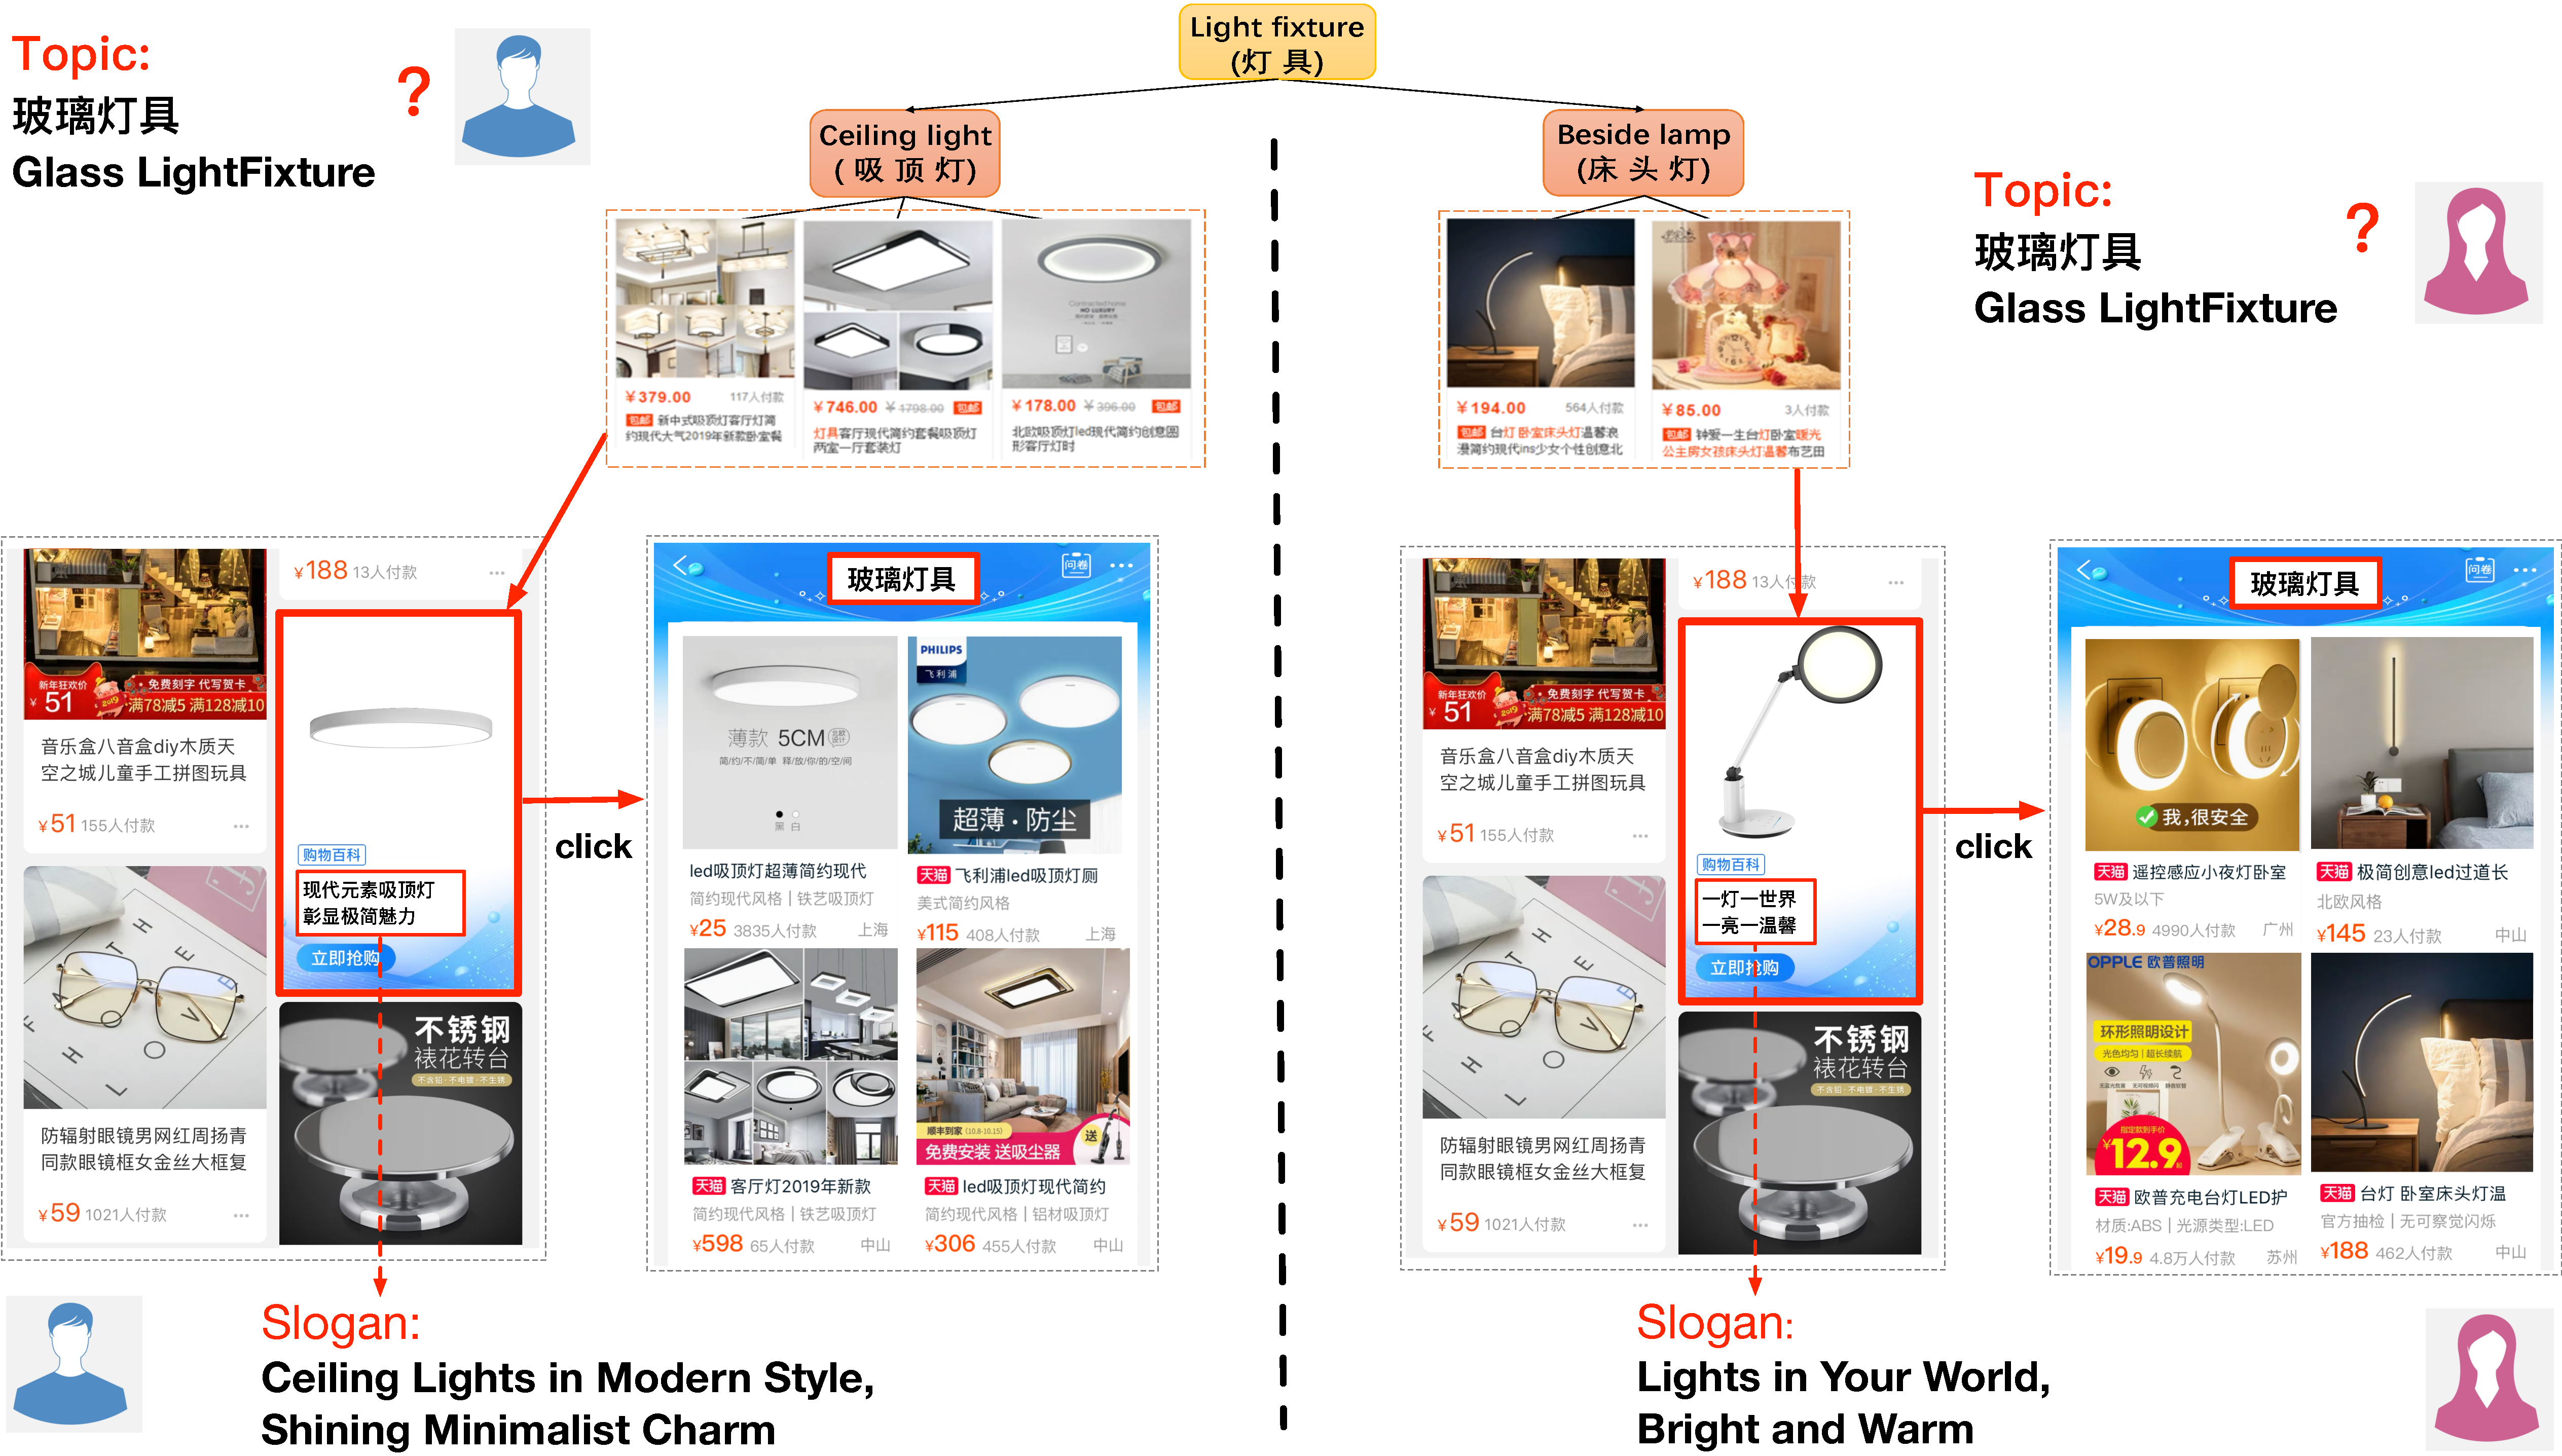
\epsfig{file=figures/cloud.eps, width=\columnwidth}
	\caption{Three real examples of user-needs driven recommendation.
		(a): Queries trigger concept cards in semantic search. (b): Display concepts directly to users as cards with a set of related items. (c): Concepts act as explanations in search and recommendation.
	}
	\label{fig:cloud}
\end{figure}

\begin{itemize}
	%\itemsep0em
	\item We claim that current ontologies in e-commerce platforms are unable to represent and understand actual user needs well and therefore prevent shopping experience from being more intelligent. To bridge the semantic gap in between, we formally define user needs in e-commerce and propose to build an end-to-end large comprehensive knowledge graph called ``AliCoCo'', where the ``concept'' nodes can explicitly represent various shopping needs for users.
	\item To construct such a large-scale knowledge graph, we adopt a semi-automatic way by combining both machine learning efforts and manual efforts together. We detailed introduce the four-layer structure of AliCoCo and five non-trivial technical components. For each component, we formulate the problem, point out the challenge, describe effective solutions and give thorough evaluations.
	\item AliCoCo is already gone into production in Alibaba, the largest e-commerce platform in China. It benefits a series of applications including search and recommendation.
	We believe the idea of user needs understanding can be further applied in more e-commerce productions. There is ample room for imagination and further innovation in ``user-needs driven'' e-commerce.
\end{itemize}

The rest of paper is organized as follows:
First we give an overview
of AliCoCo (\secref{sec:overview}), then present how we construct each of the four layers:
Taxonomy (\secref{sec:taxonomy}), Primitive Concepts (\secref{sec:primitive}), E-commerce Concepts (\secref{sec:ecommerce}), and Item Associations (\secref{sec:item}).
\secref{sec:eval} shows overall statistics of AliCoCo and evaluations of five main technical modules.
Then we discuss some successful, ongoing and potential applications in \secref{sec:application}.
\secref{sec:related} mentions related works, and finally, \secref{sec:conclusion} gives a conclusion and delineates possible future work.
